\label{sec:muroexe}

The design philosophy of MuroEXE is to use CNN as much as possible to accomplish various tasks on the robot. Because the CNN not only has advantages over traditional algorithms in accuracy, but also has uniform and regular computing mode. Therefore, a single instruction-driven CNN accelerator can speed up different tasks. The unified accelerator can reduce the use of hardware resources and make it easier to implement the robot computing system on embedded FPGA.

The framework MUROEXE is proposed to make the robotics community better use of the FPGA accelerator. As the Robot Operating System (ROS) \cite{quigley2009ros} is a popular middleware fusing different modules from different developers, MUROEXE is designed for the multi-thread scheduling method in ROS.

In ROS, a basic function is implemented as a node, and different nodes are executed in different CPU threads with little and asynchronous data communication.


\begin{figure}[t]
	\centering
    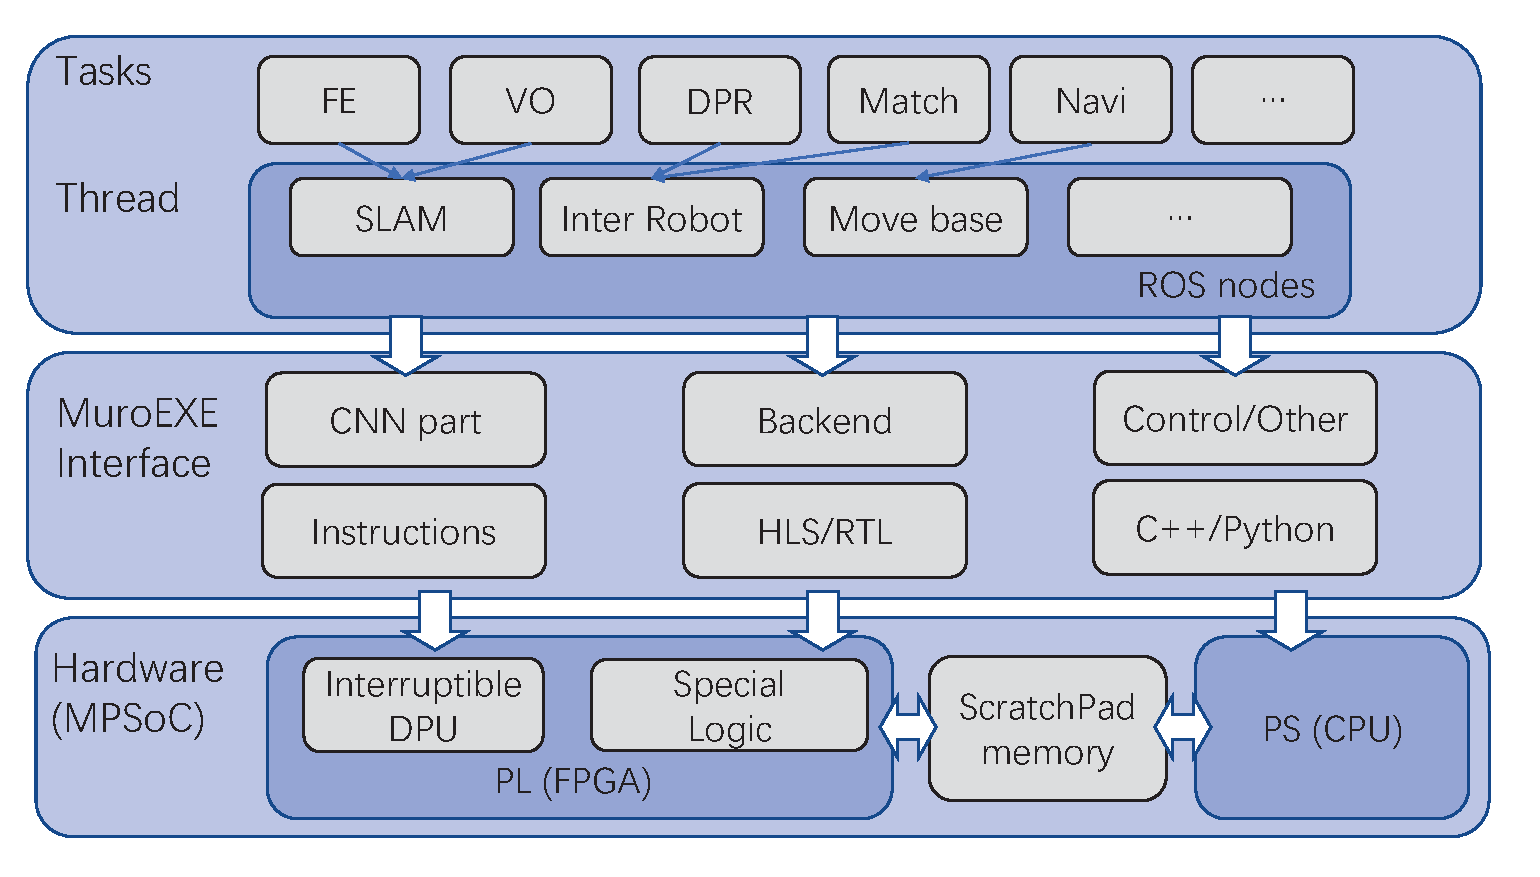
\includegraphics[width=0.99\linewidth]{fig/muroexe.eps}
    \caption{ Overview of the MUROEXE framework. Each ROS node is a separate thread. The CNNs in different ROS nodes are deployed onto the interruptible accelerator. The post-processing in the ROS nodes can accelerated by the RTL/HLS modules. The hardware modules for post-processing and the CNN accelerator share data through scrachpad memory. }
	\label{fig:muroexe}
\end{figure}